\subsection{Loading datasets with more than 8 masses}
\setcounter{step}{0}

\goldbox{}
During a~typical NanoSIMS measurement, at most 8~different ionic species are recorded: 7~different isotopes, and secondary electrons (normally denoted as \ttt{Esi}). This explains the visual design of LANS, which contains 8~fields for \lanstf{detected masses}. However, NanoSIMS instrument can operate in a~so-called peak-switching mode, which allows quasi-simultaneous detection of up to 15~different ionic species ($2\times 7$ different isotopes and \ttt{Esi}). This section explains how to use LANS to analyze datasets containing counts of more than 8~ionic species.
\tcbe

\noindent
This feature was added to LANS based on a~request from Dr.~Hryhoryi Stryhanyuk (UFZ Leipzig). In the example below, we use one of the datasets acquired in his lab to illustrate the approach: \ttt{2022-01-25-OPG\_1.im.zip}.

\vskip0.5\baselineskip

\sbx{Load the raw dataset.}

\nbx{This is done in the usual way, as for any other dataset. Based on the structure of the data within the binary file, LANS will automatically recognize that it was acquired in a~peak-switching mode and rearrange the data accordingly.} 

\nnb{%
An example of the output generated during loading is shown here:
\begin{center}
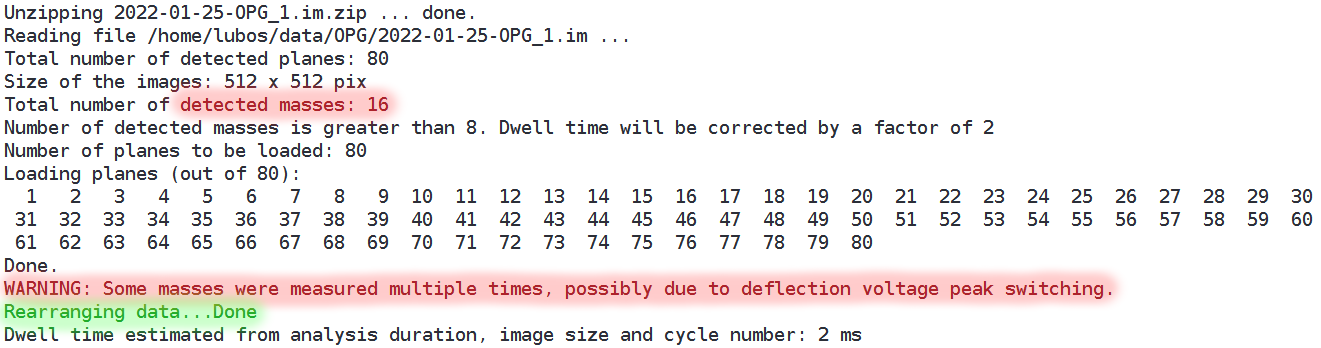
\includegraphics[scale=0.34]{figs8/LANS-8plus-load}
\end{center}
}

\s{After loading, it is a~good idea to first find out which ions were actually detected. This is best done by selecting \lans{Input} $\ra$ \lans{Autoscale plane images}.}

\nnb{In this example, LANS indicated that data from 16 masses were detected (see output above). However, some of the masses were recorded repeatedly because not all detectors used peak-switching during ion detection. In fact, the number of \emph{different} ionic species detected in this example was~12: ${}^{16}\mathrm{O}{}^1\mathrm{H}$, ${}^{16}\mathrm{O}{}^2\mathrm{H}$, ${}^{12}\mathrm{C}_2$, ${}^{12}\mathrm{C}{}^{13}\mathrm{C}$, ${}^{12}\mathrm{C}{}^{14}\mathrm{N}$, secondary electrons (\ttt{Esi}), ${}^{12}\mathrm{C}{}^{15}\mathrm{N}$, ${}^{32}\mathrm{S}$, ${}^{12}\mathrm{C}_2{}^{1}\mathrm{H}$, ${}^{12}\mathrm{C}_2{}^{2}\mathrm{H}$, ${}^{13}\mathrm{C}{}^{14}\mathrm{N}$, and ${}^{31}\mathrm{P}{}^{1}\mathrm{H}$, as follows from the output in the Matlab console:
\begin{center}
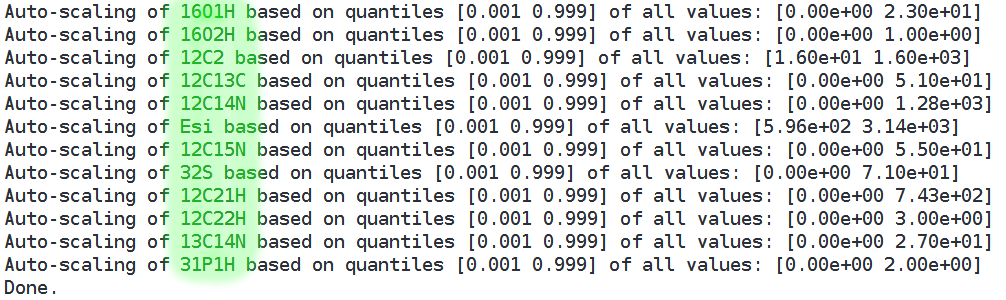
\includegraphics[scale=0.34]{figs8/LANS-8plus-autoscale}
\end{center}}

\nb{It is important the realize that due to the limited number of fields dedicated to detected \lanstf{masses} in the LANS user interface (maximum~8), all of these ionic species \emph{cannot} be displayed in the list. Indeed, only the first 8~masses are included in the list. Nevertheless, they \emph{are} registered internally within the list of detected masses and can therefore be used in any of the \lanstf{expressions} (see below).}

\sbx{Select \lans{Input} $\ra$ \lans{Display plane images for all masses} to view the raw ion counts, plane by plane.}

\nnb{Note that some masses only show non-zero counts in \emph{every second plane}. This is because the specific detectors used peak switching to alternately detect two ionic species at the same nominal mass. In this example, it concerns the following pairs: ${}^{12}\mathrm{C}{}^{13}\mathrm{C}$ \& ${}^{12}\mathrm{C}_2{}^{1}\mathrm{H}$ at nominal mass~25, ${}^{12}\mathrm{C}{}^{14}\mathrm{N}$ \& ${}^{12}\mathrm{C}_2{}^{2}\mathrm{H}$ at nominal mass~26, ${}^{12}\mathrm{C}{}^{15}\mathrm{N}$ \& ${}^{13}\mathrm{C}{}^{14}\mathrm{N}$ at nominal mass~27, and ${}^{32}\mathrm{S}$ \& ${}^{31}\mathrm{P}{}^{1}\mathrm{H}$ at nominal mass~32 (Fig.~\ref{fig:LANS-8plus-frames}A--B).}

\begin{figure}[!ht]
\centering
\begin{tabular}{c}
A: 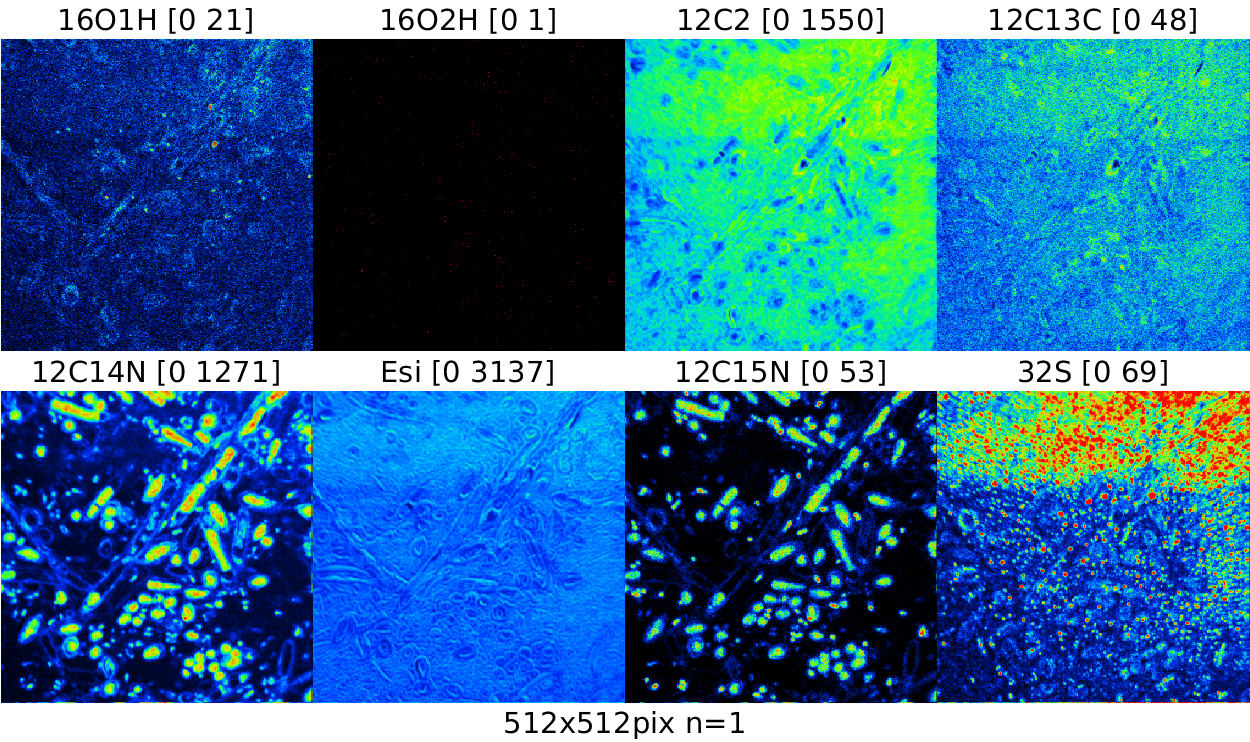
\includegraphics[scale=0.43, valign=t]{figs8/m-001}
\\
B: 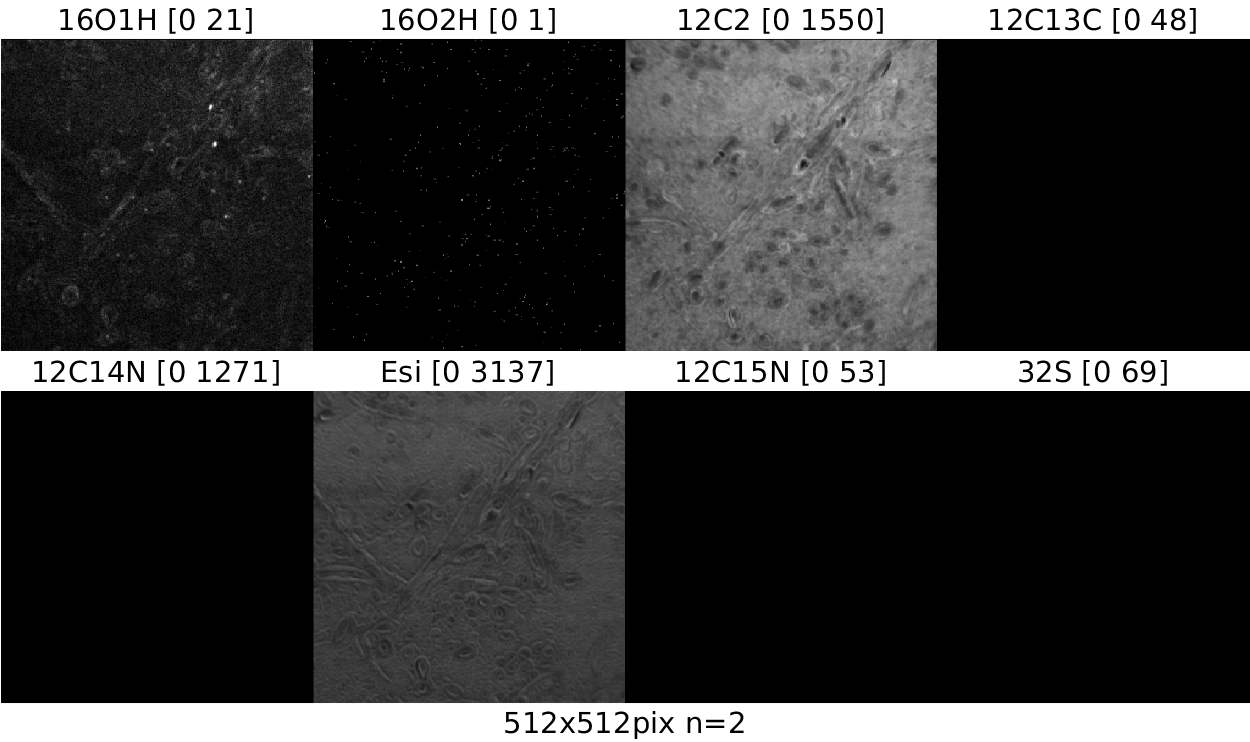
\includegraphics[scale=0.43, valign=t]{figs8/m-002}
\\
C: 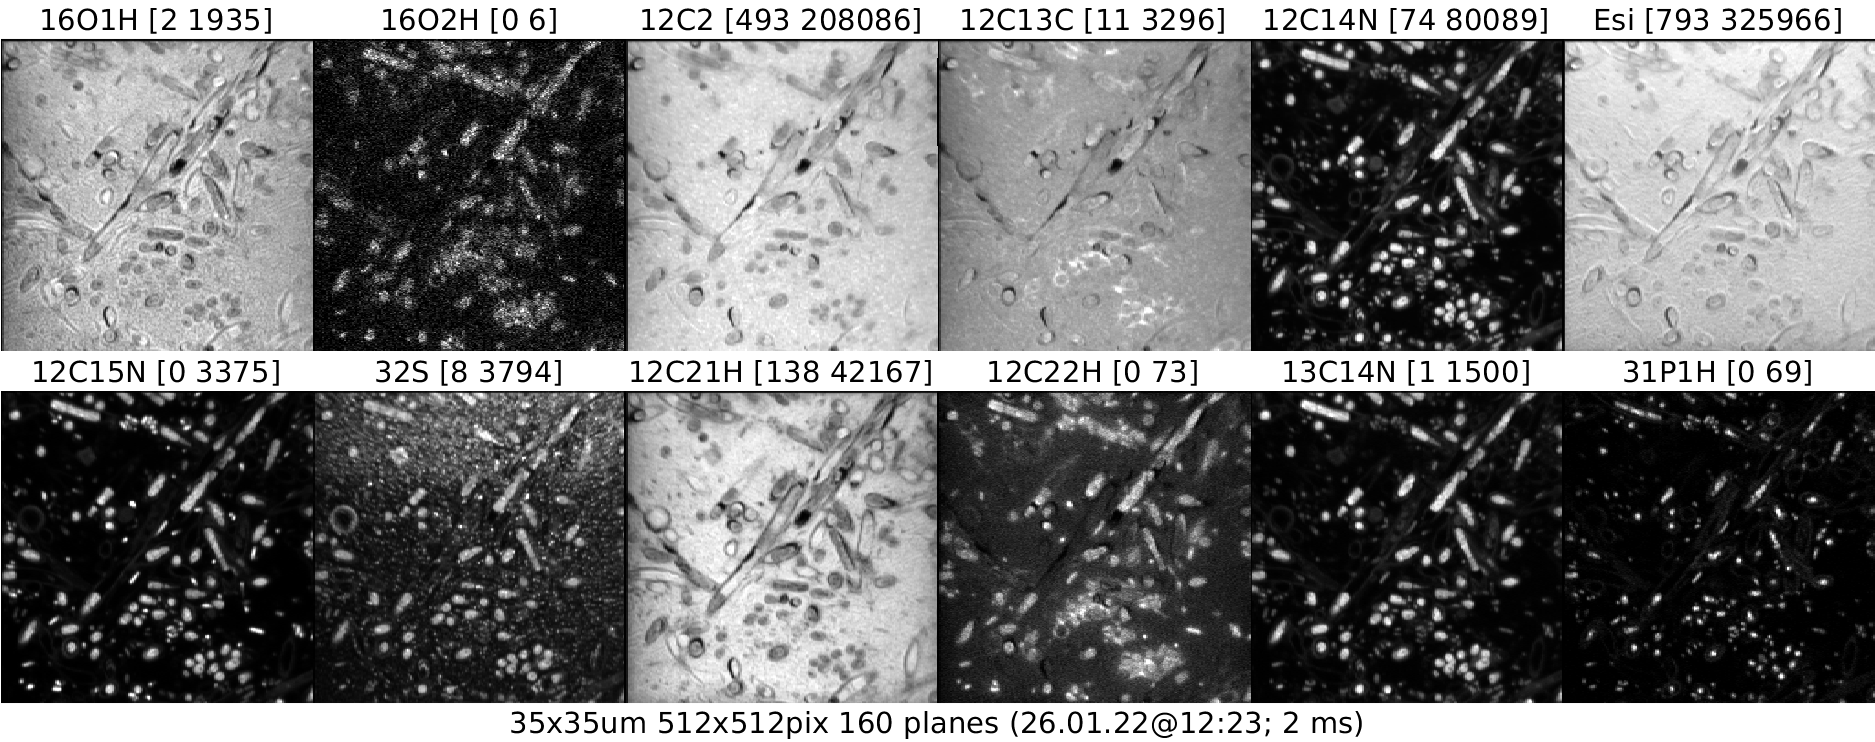
\includegraphics[width=0.86\textwidth, valign=t]{figs8/2022-01-25-OPG-all}
\end{tabular}
\caption{\label{fig:LANS-8plus-frames}%
Example of raw data acquired via peak-switching mode. Panels (A--B) show ion counts in the first two planes, as obtained by selecting \lans{Input} $\ra$ \lans{Display plane images for all masses}. Note that only the first 8~masses are displayed in this way, although a~total of 12~different masses were detected. This is due to the limitation of the  graphical interface of LANS. This limitation, however, does not impede further analysis of the data by LANS. Panel C shows the accumulated ion count images, as obtained by selecting  \lans{Input} $\ra$ \lans{Display accumulated images for all masses}. In this case, all 12~detected masses are displayed side-by-side.}
\end{figure}

\s {While viewing the detected ions in the previous step, identify suitable mass that can be used as a~\lanstf{Base mass for alignment} and type it into the corresponding text field.}

\nbx{Clearly, this mass should have non-zero ion counts in \emph{every} plane to yield valid drift correction information.}

\nnb{In this example, it cannot be \ttt{12C14N}. Instead, \ttt{Esi} is a good candidate, as it is detected in every plane and has sufficiently high counts and contrast in individual planes. \ttt{12C2} could be another good candidate. }

\sbx{Select \lans{Input} $\ra$ \lans{Accumulate plane images} to accumulate drift-corrected ion images.}

\nnb{As usual, the \lanscb{Align images when accumulating} checkbox needs to be checked if you want to perform drift correction during accumulation of planes.}

\s{Select \lans{Input} $\ra$ \lans{Autoscale accumulated images} and then  \lans{Input} $\ra$ \lans{Displayed accumulated images} \lans{for all masses} to autoscale and display accumulated images for all masses.} 

\nnb{In contrast to the display of individual planes, this will visualize accumulated images for \emph{all} detected masses, providing a~full view of the raw data (Fig.~\ref{fig:LANS-8plus-frames}C).}
 
\sbx{Proceed as described in Section~\ref{sec:level1} to analyze ion counts, ion count ratios, or conduct other types of analysis.}

\nnb{Examples of the output generated for this type of data are shown in Fig.~\ref{fig:LANS-8plus-ratios}.}

\nbx{When analyzing data with more than 8~masses, you need to pay special attention to the following: If you want to display (and export) ion count images for masses that are \emph{not} displayed in the list of 8~detected masses, you need to type the name of the mass in the \lanstf{expression} field for the \bb{ratio}, as illustrated in Fig.~\ref{fig:LANS-8plus-extra-masses}, adjust the scale, and then select \lans{Output} $\ra$ \lans{Display ratios}. For example, you need to proceed in this way to display images of ${}^{12}\mathrm{C}_2{}^{1}\mathrm{H}$ (\ttt{12C21H}), ${}^{12}\mathrm{C}_2{}^{2}\mathrm{H}$ (\ttt{12C22H}), ${}^{13}\mathrm{C}{}^{14}\mathrm{N}$ (\ttt{13C14N}), or ${}^{31}\mathrm{P}{}^{1}\mathrm{H}$ (\ttt{31P1H}).}

\nb{Additionally, you need to pay extra attention when defining \lanstf{expressions} for isotope ratios. For example, if the molecular ions of ${}^{12}\mathrm{C}{}^{13}\mathrm{C}$ and ${}^{12}\mathrm{C}_2$ were detected in every plane, the correct expression for obtaining the atomic ${}^{13}\mathrm{C}/{}^{12}\mathrm{C}$ isotope ratio would be \ttt{0.5*12C13C/12C2}. However, because in this example the molecular ions of ${}^{12}\mathrm{C}{}^{13}\mathrm{C}$ were only detected in every second plane, while the molecular ions of ${}^{12}\mathrm{C}_2$ were detected in every plane, the correct expression for the ${}^{13}\mathrm{C}/{}^{12}\mathrm{C}$ isotope ratio is \ttt{12C13C/12C2}.}

\sbx{When finishing the analysis, don't forget to save the preferences by selecting \lans{Preferences} $\ra$ \lans{Store preferences}.}

\def\scf{0.36}
\begin{figure}[!h]
\centering
\begin{tabular}{ccc}
A & B & C \\
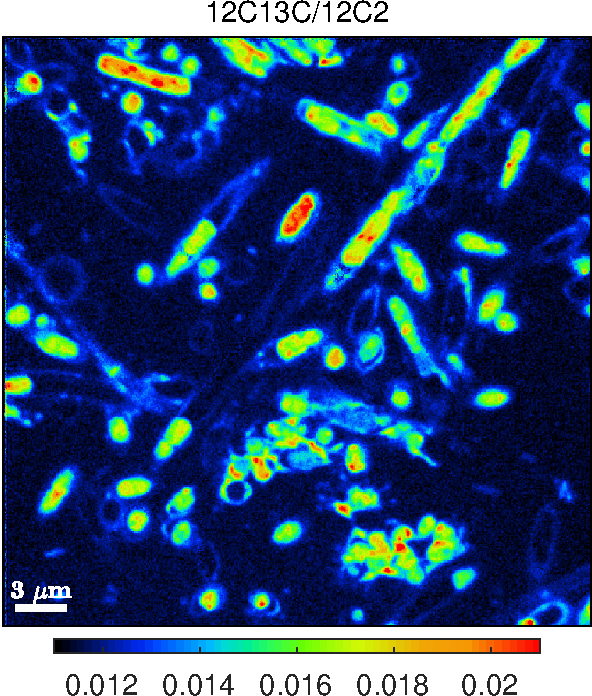
\includegraphics[scale=\scf, valign=t]{figs8/12C13C-12C2}
&
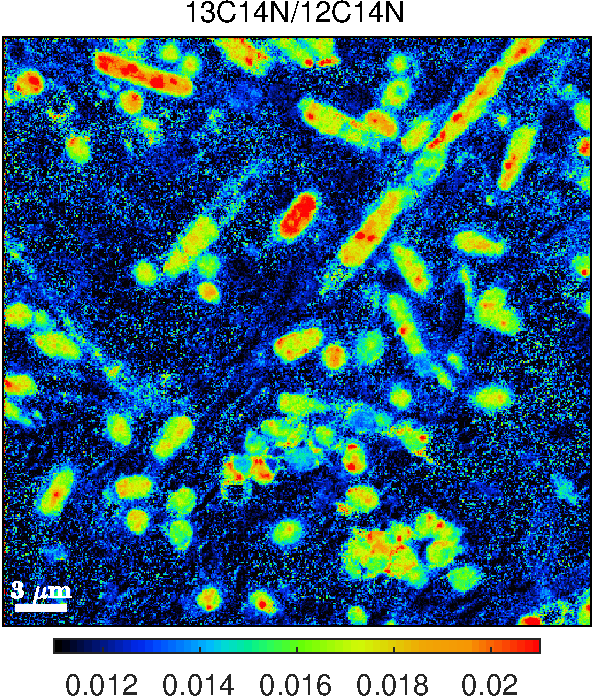
\includegraphics[scale=\scf, valign=t]{figs8/13C14N-12C14N}
&
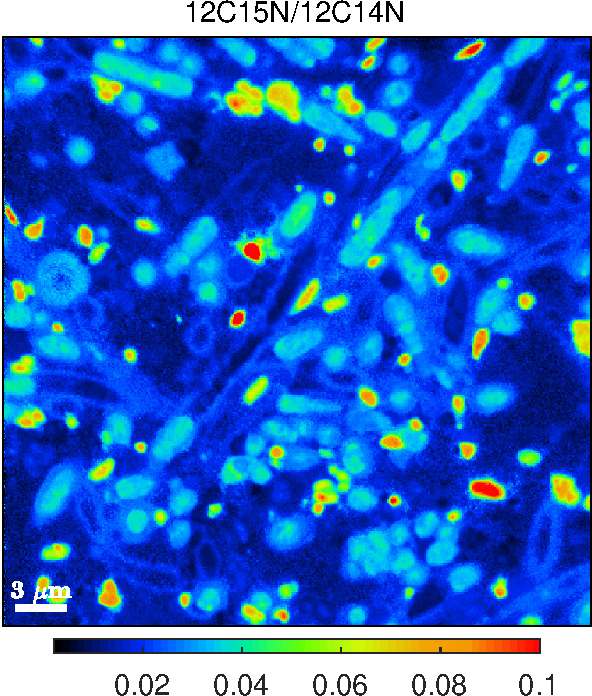
\includegraphics[scale=\scf, valign=t]{figs8/12C15N-12C14N}
\\
D & E & F\\
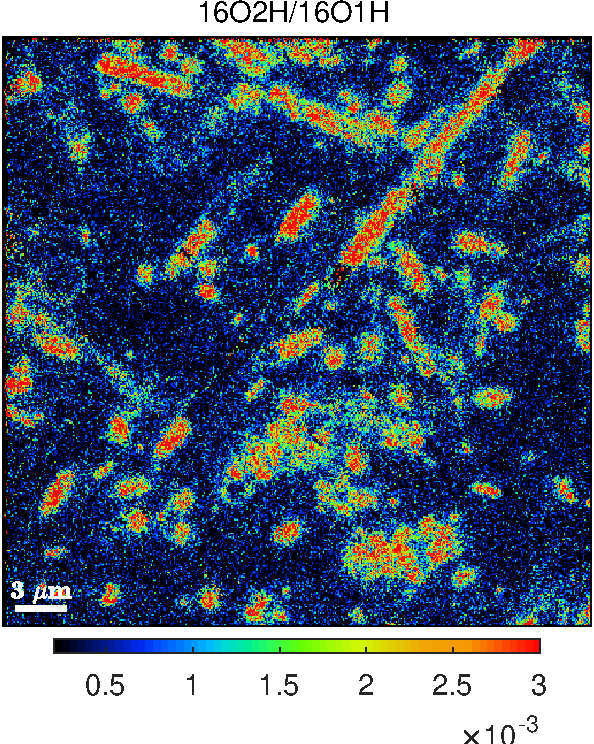
\includegraphics[scale=\scf, valign=t]{figs8/16O2H-16O1H}
&
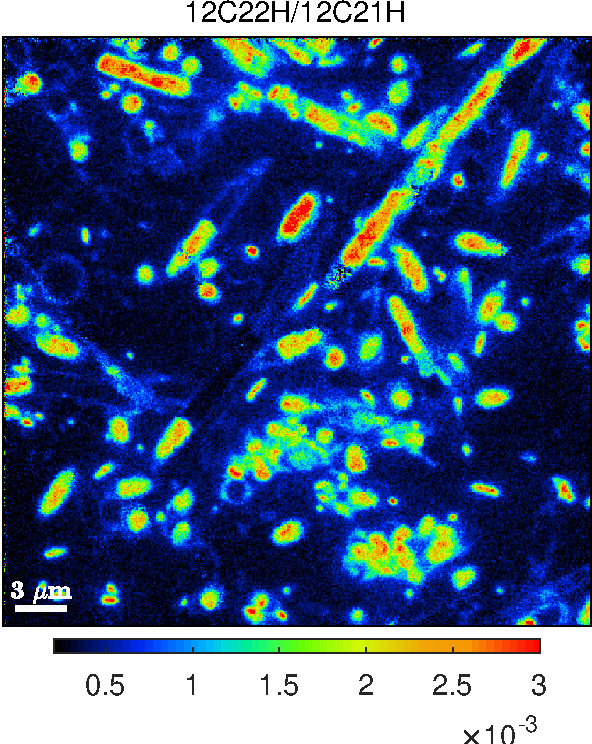
\includegraphics[scale=\scf, valign=t]{figs8/12C22H-12C21H}
&
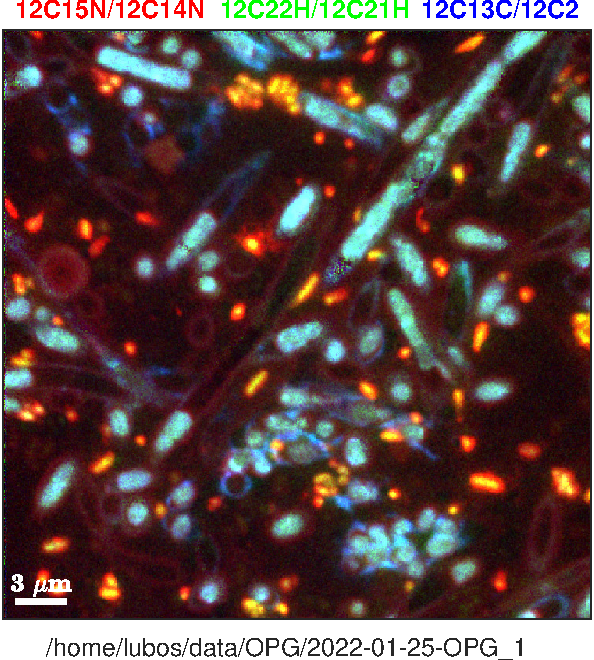
\includegraphics[scale=\scf, valign=t]{figs8/12C15N-12C14N-vs-12C22H-12C21H-vs-12C13C-12C2-rgb}
\end{tabular}
\caption{\label{fig:LANS-8plus-ratios}%
Examples of isotope ratio images derived from data collected via peak-switching mode, illustrating the power of this measurement approach for multi-isotope imaging mass spectrometry. Panels (A--B) show the ${}^{13}\mathrm{C}/{}^{12}\mathrm{C}$ isotope ratio obtained from two different ion pairs: ${}^{12}\mathrm{C}{}^{13}\mathrm{C}$ \&\ ${}^{12}\mathrm{C}_2$ and ${}^{13}\mathrm{C}{}^{14}\mathrm{N}$ \&\ ${}^{12}\mathrm{C}{}^{14}\mathrm{N}$. Panel C shows the ${}^{15}\mathrm{N}/{}^{14}\mathrm{N}$ isotope ratio obtained from the ion pair ${}^{12}\mathrm{C}{}^{15}\mathrm{N}$ \&\ ${}^{12}\mathrm{C}{}^{14}\mathrm{N}$. Panels (D--E) show the ${}^{2}\mathrm{H}/{}^{1}\mathrm{H}$ isotope ratio obtained from two different ion pairs: ${}^{16}\mathrm{O}{}^{2}\mathrm{H}$ \&\ ${}^{16}\mathrm{O}{}^{1}\mathrm{H}$ and ${}^{12}\mathrm{C}_2{}^{2}\mathrm{H}$ \&\ ${}^{12}\mathrm{C}_2{}^{1}\mathrm{H}$. Panel F shows an RGB overlay between the three isotope ratios: ${}^{15}\mathrm{N}/{}^{14}\mathrm{N}$ (red), ${}^{2}\mathrm{H}/{}^{1}\mathrm{H}$ (green), and ${}^{13}\mathrm{C}/{}^{12}\mathrm{C}$ (blue).}
\end{figure}

\begin{figure}[!hb]
\centering
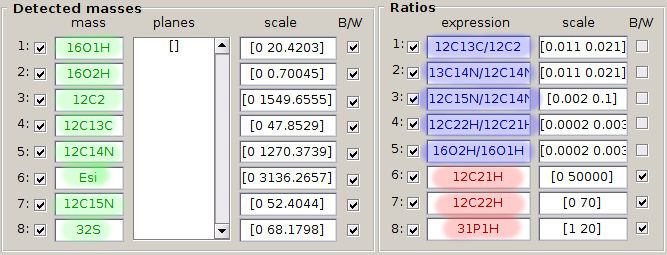
\includegraphics[scale=0.42, valign=t]{figs8/LANS-8plus-masses-ratios}
\caption{\label{fig:LANS-8plus-extra-masses}%
Processing of data acquired using peak-switching mode. Text fields on the left only contain the first 8~masses present in the dataset (marked by green). If you want to display the other masses in the dataset, you need to type their name in one of the \lanstf{expression} text fields on the right (marked by red), adjust the scale, and then select \lans{Output} $\ra$ \lans{Display ratios}. Similarly, you can use the names in \lanstf{expressions} to calculate ion count ratios (marked by blue).}
\end{figure}

